
\documentclass{article}
\usepackage{graphicx}
\usepackage{booktabs}
\usepackage{float}
\usepackage{siunitx}
\usepackage{geometry}
\geometry{margin=2.5cm}

\title{Network Simulation Analysis Report}
\author{Generated Report}
\date{\today}

\begin{document}
\maketitle

\section{Introduction}
This report presents the analysis of network simulation results using various parameters including node count, packets per second, and node speed.

\section{Parameter Analysis}
\subsection{Single Parameter Impact}
The following figures show how individual parameters affect network metrics while keeping other parameters constant.

\begin{figure}[h]
\centering
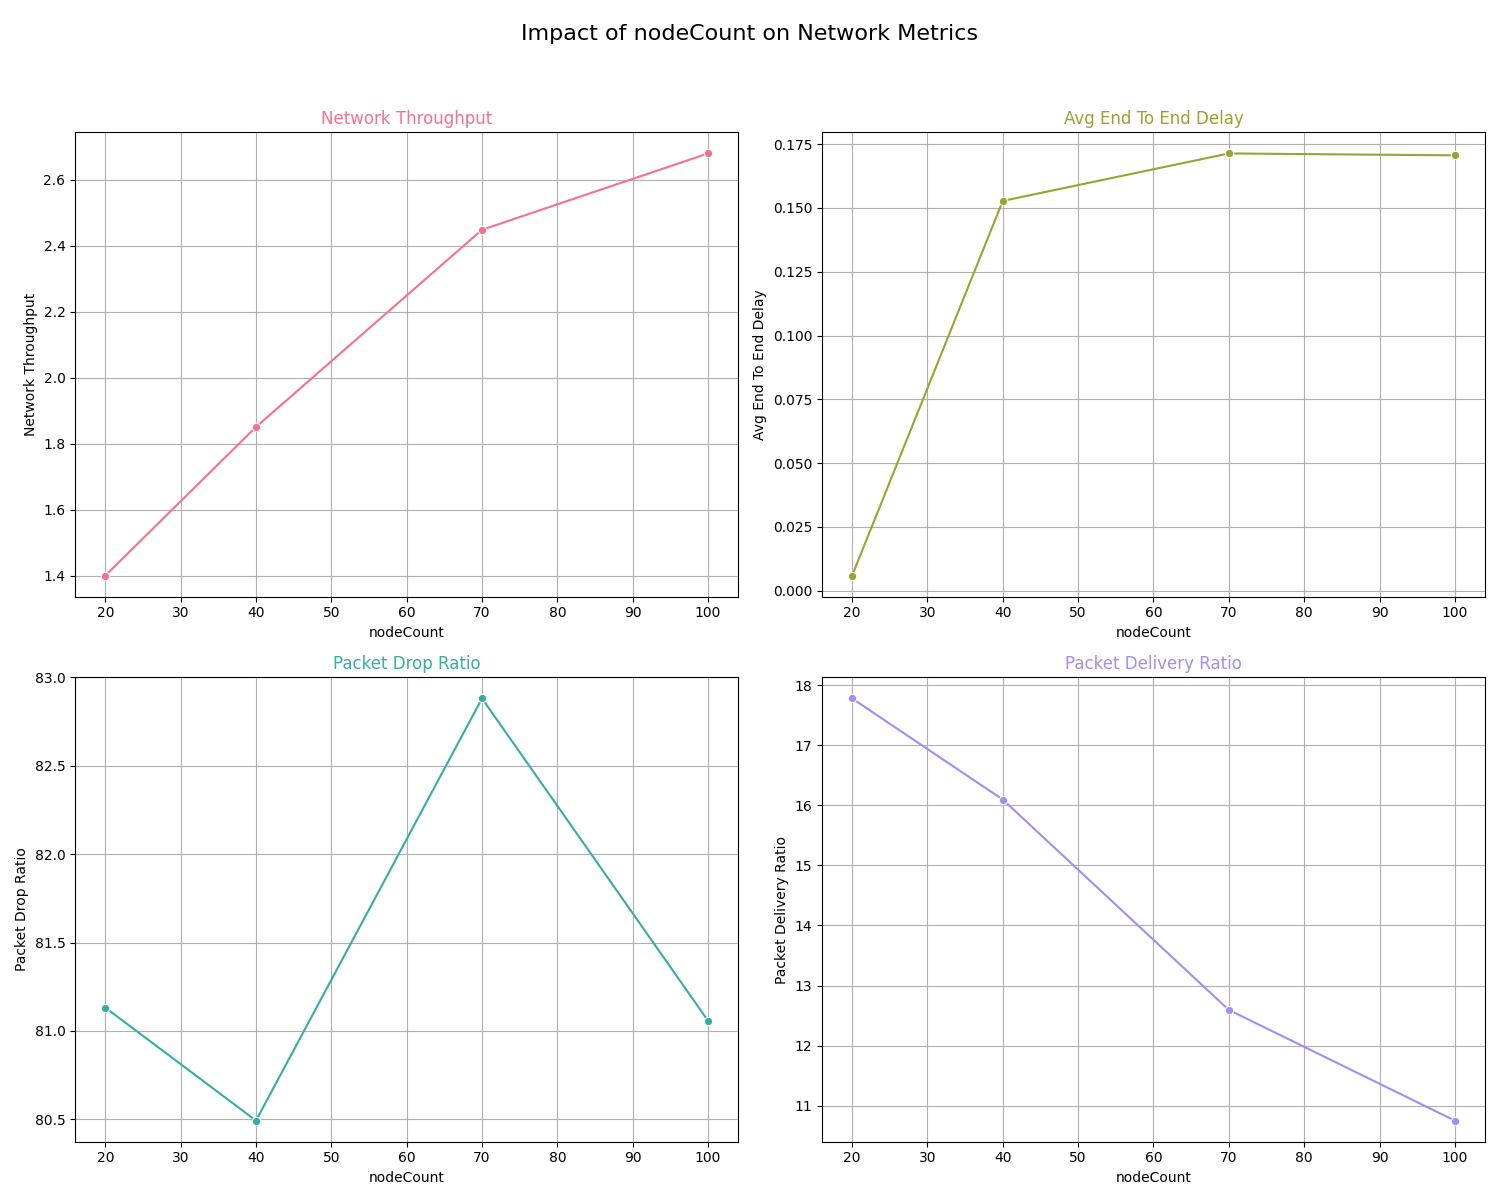
\includegraphics[width=0.8\textwidth]{plots/task-1/single-input-params/analysis_nodeCount}
\caption{Impact of Node Count on Network Metrics}
\end{figure}

\begin{figure}[h]
\centering
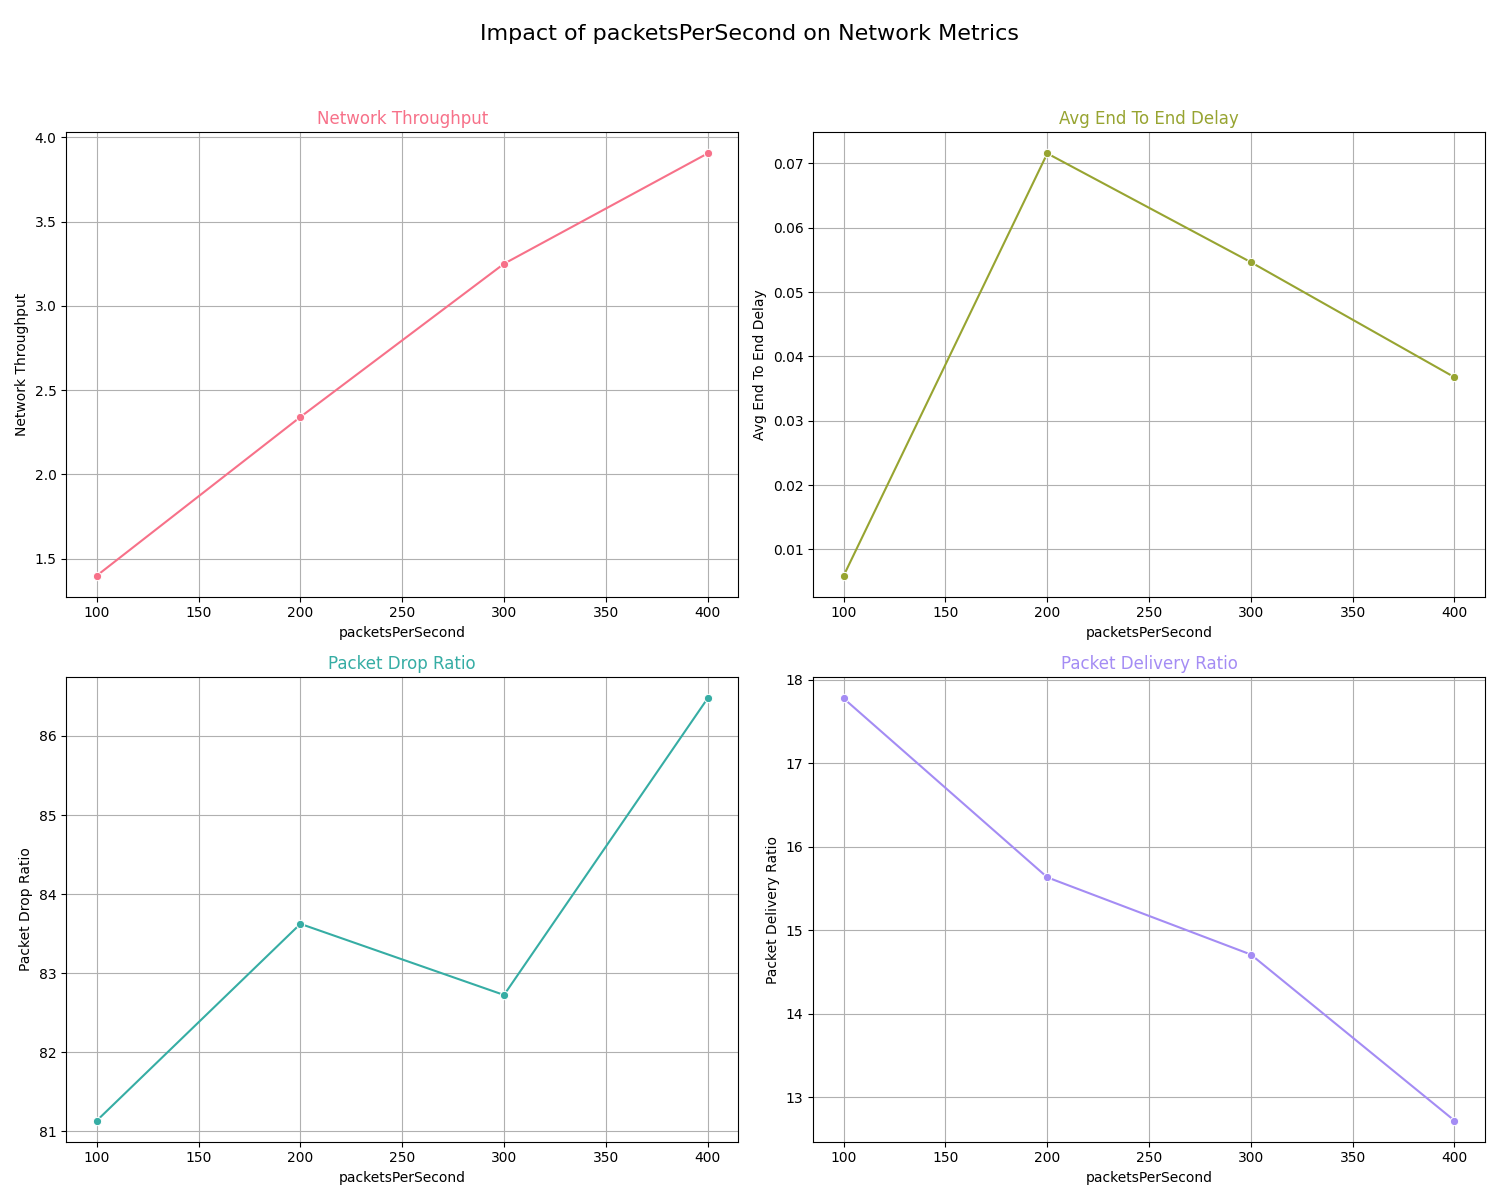
\includegraphics[width=0.8\textwidth]{plots/task-1/single-input-params/analysis_packetsPerSecond}
\caption{Impact of Packets Per Second on Network Metrics}
\end{figure}

\begin{figure}[h]
\centering
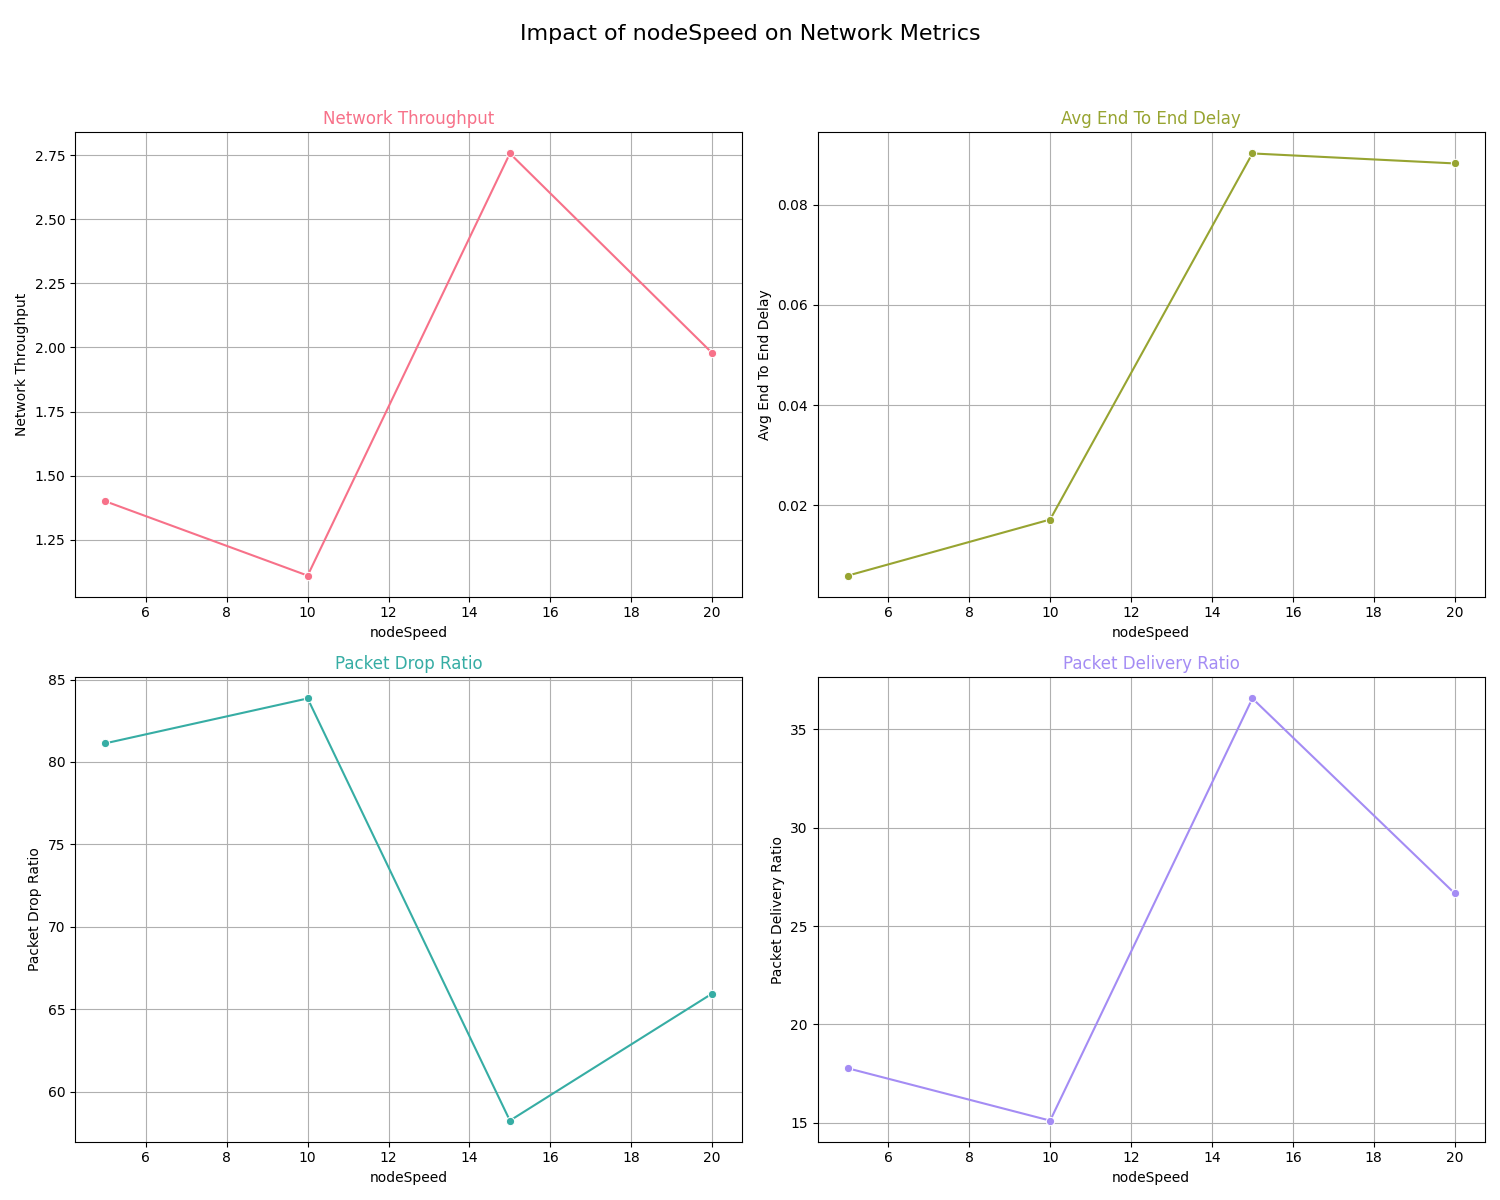
\includegraphics[width=0.8\textwidth]{plots/task-1/single-input-params/analysis_nodeSpeed}
\caption{Impact of Node Speed on Network Metrics}
\end{figure}

\subsection{Parameter Interactions}
Heat maps showing the interaction between pairs of parameters:

\begin{figure}[h]
\centering
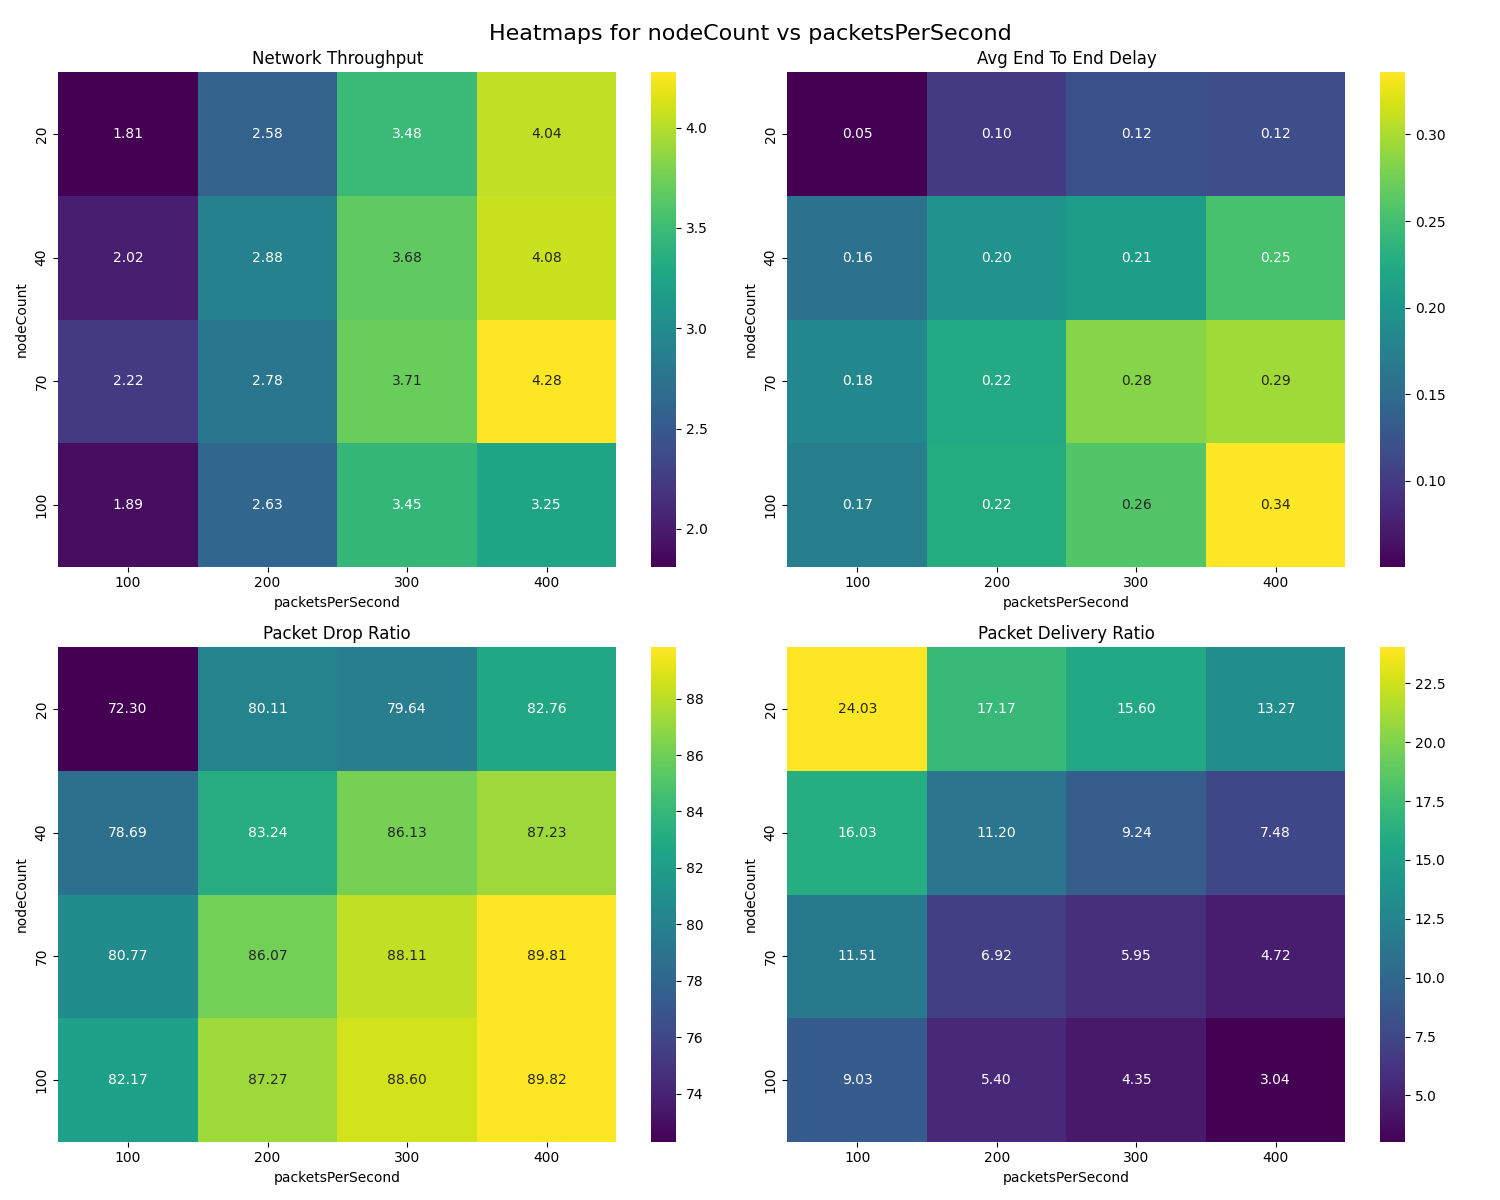
\includegraphics[width=0.8\textwidth]{plots/task-1/two-params-heatmaps/heatmap_nodeCount_packetsPerSecond}
\caption{Heatmap: Node Count vs Packets Per Second}
\end{figure}

\begin{figure}[h]
\centering
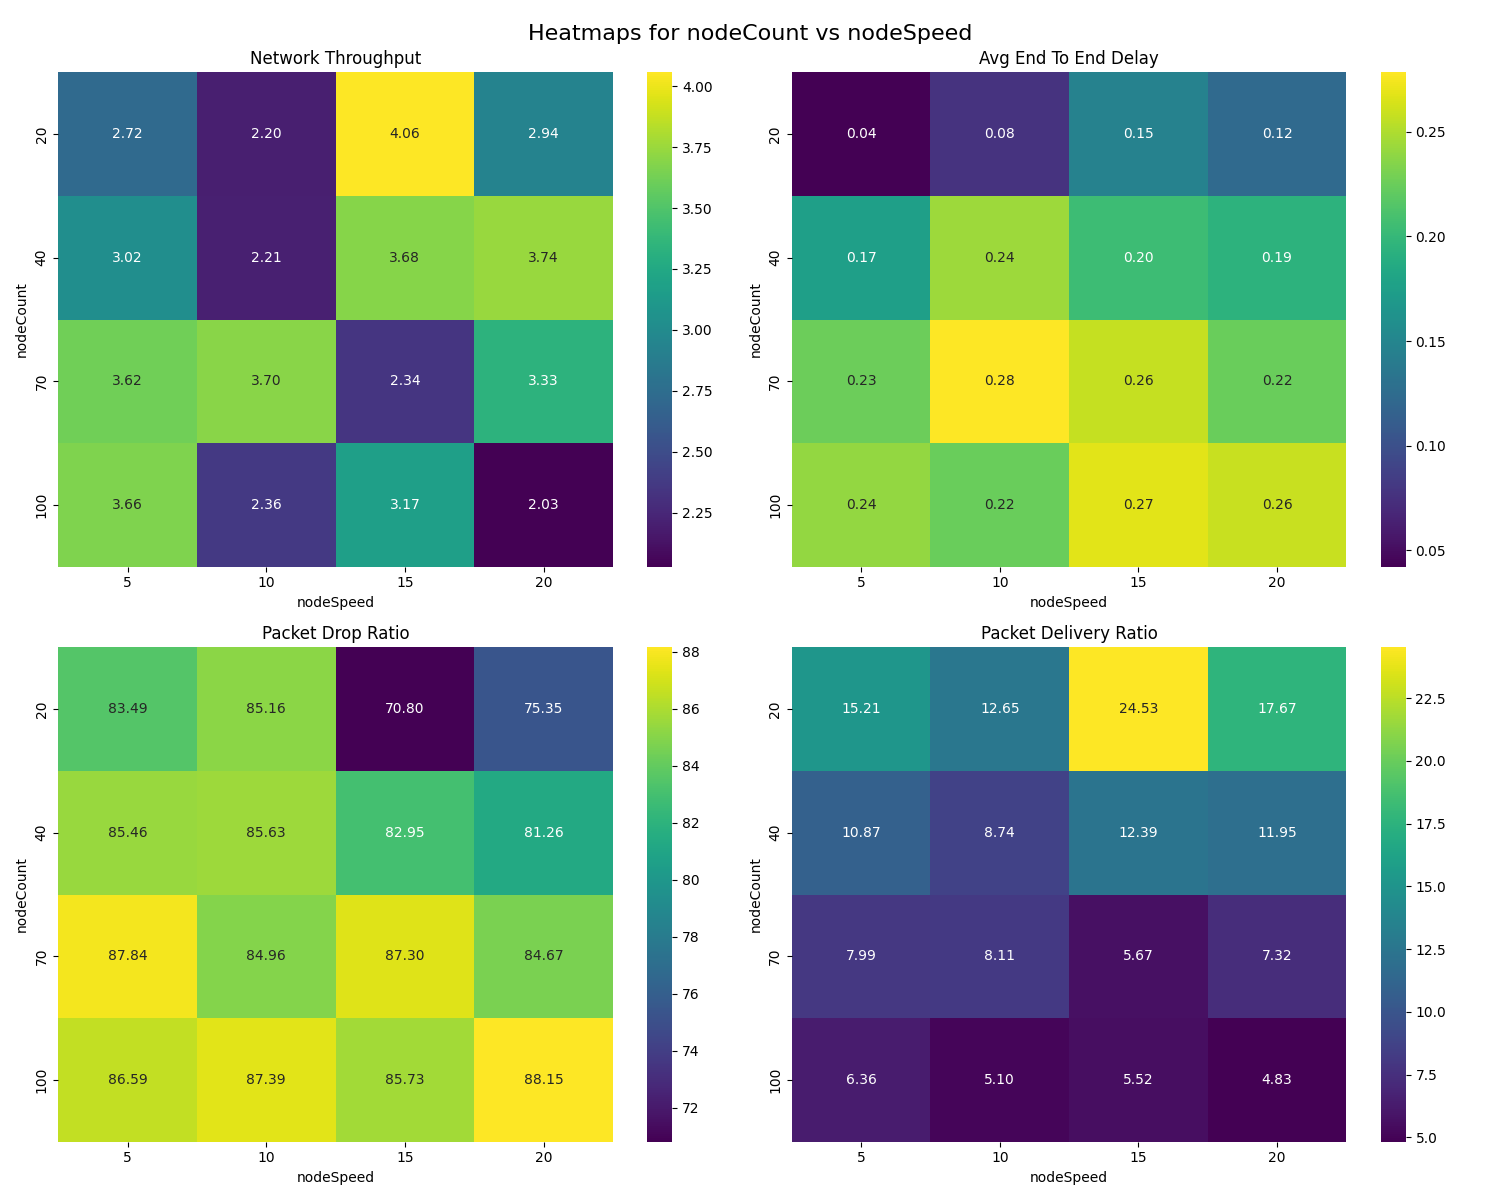
\includegraphics[width=0.8\textwidth]{plots/task-1/two-params-heatmaps/heatmap_nodeCount_nodeSpeed}
\caption{Heatmap: Node Count vs Node Speed}
\end{figure}

\begin{figure}[h]
\centering
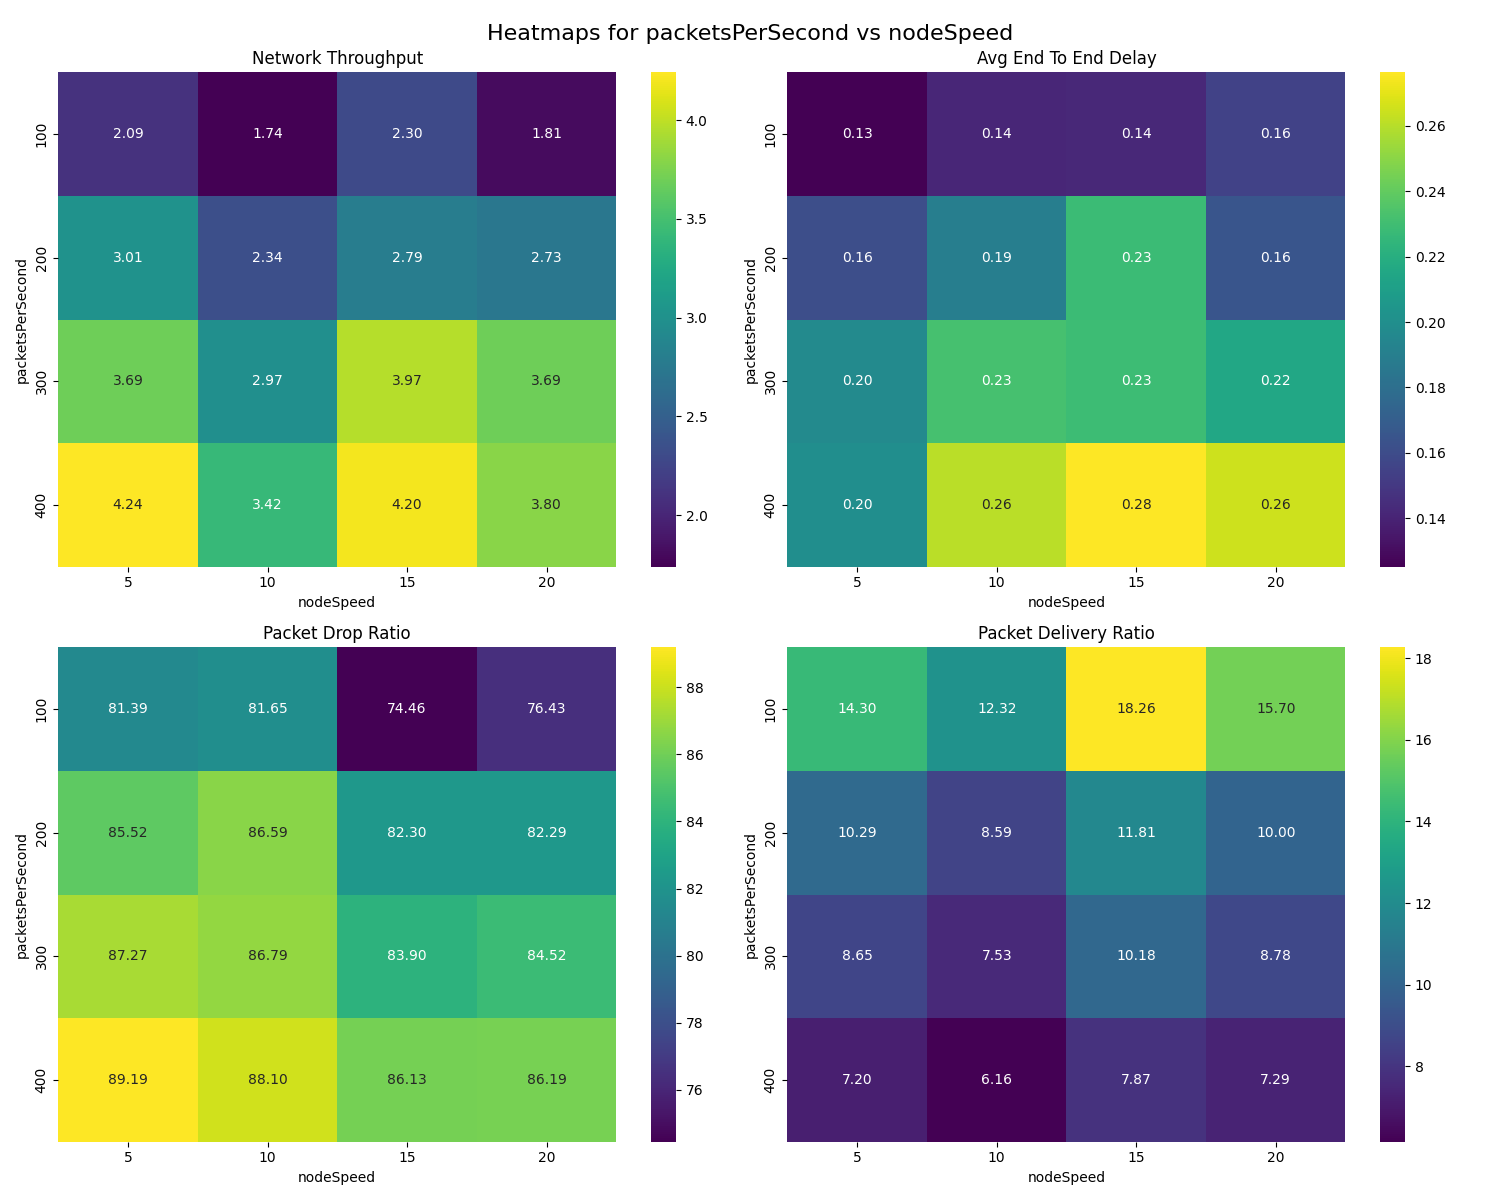
\includegraphics[width=0.8\textwidth]{plots/task-1/two-params-heatmaps/heatmap_packetsPerSecond_nodeSpeed}
\caption{Heatmap: Packets Per Second vs Node Speed}
\end{figure}

\section{Detailed Results}
The following table shows the complete simulation results. Bold values indicate maximum values for each metric.
\begin{table}[h]
\centering\small
\caption{Complete Simulation Results}
\begin{tabular}{l l l l l l l}
\toprule
Node Count & PPS & Speed & Throughput & End-to-End Delay & Drop Ratio & Delivery Ratio \\
\midrule
100 & 100 & 10 & 1.66 & 0.18 & 0.83 & 0.09 \\
100 & 100 & 15 & 2.24 & 0.16 & 0.80 & 0.09 \\
100 & 100 & 20 & 0.99 & 0.18 & 0.84 & 0.08 \\
100 & 100 & 5 & 2.68 & 0.17 & 0.81 & 0.11 \\
100 & 200 & 10 & 1.88 & 0.21 & 0.88 & 0.05 \\
100 & 200 & 15 & 2.68 & 0.26 & 0.86 & 0.05 \\
100 & 200 & 20 & 2.44 & 0.22 & 0.88 & 0.05 \\
100 & 200 & 5 & 3.50 & 0.20 & 0.86 & 0.06 \\
100 & 300 & 10 & 3.04 & 0.22 & 0.88 & 0.04 \\
100 & 300 & 15 & 4.31 & 0.24 & 0.88 & 0.05 \\
100 & 300 & 20 & 2.77 & 0.31 & 0.90 & 0.04 \\
100 & 300 & 5 & 3.66 & 0.26 & 0.89 & 0.05 \\
100 & 400 & 10 & 2.87 & 0.29 & 0.90 & 0.03 \\
100 & 400 & 15 & 3.43 & \textbf{0.40} & 0.89 & 0.03 \\
100 & 400 & 20 & 1.91 & 0.33 & 0.91 & 0.02 \\
100 & 400 & 5 & 4.81 & 0.33 & 0.90 & 0.04 \\
20 & 100 & 10 & 1.11 & 0.02 & 0.84 & 0.15 \\
20 & 100 & 15 & 2.76 & 0.09 & 0.58 & \textbf{0.37} \\
20 & 100 & 20 & 1.98 & 0.09 & 0.66 & 0.27 \\
20 & 100 & 5 & 1.40 & 0.01 & 0.81 & 0.18 \\
20 & 200 & 10 & 1.80 & 0.03 & 0.87 & 0.12 \\
20 & 200 & 15 & 3.73 & 0.18 & 0.72 & 0.25 \\
20 & 200 & 20 & 2.45 & 0.11 & 0.78 & 0.16 \\
20 & 200 & 5 & 2.34 & 0.07 & 0.84 & 0.16 \\
20 & 300 & 10 & 2.74 & 0.13 & 0.84 & 0.13 \\
20 & 300 & 15 & 4.75 & 0.16 & 0.75 & 0.21 \\
20 & 300 & 20 & 3.20 & 0.14 & 0.77 & 0.14 \\
20 & 300 & 5 & 3.25 & 0.05 & 0.83 & 0.15 \\
20 & 400 & 10 & 3.16 & 0.13 & 0.86 & 0.11 \\
20 & 400 & 15 & 5.00 & 0.15 & 0.79 & 0.16 \\
20 & 400 & 20 & 4.11 & 0.15 & 0.80 & 0.14 \\
20 & 400 & 5 & 3.90 & 0.04 & 0.86 & 0.13 \\
40 & 100 & 10 & 1.54 & 0.19 & 0.81 & 0.13 \\
40 & 100 & 15 & 2.39 & 0.13 & 0.78 & 0.18 \\
40 & 100 & 20 & 2.29 & 0.16 & 0.76 & 0.17 \\
40 & 100 & 5 & 1.85 & 0.15 & 0.80 & 0.16 \\
40 & 200 & 10 & 2.05 & 0.26 & 0.85 & 0.09 \\
40 & 200 & 15 & 3.52 & 0.19 & 0.83 & 0.13 \\
40 & 200 & 20 & 3.30 & 0.16 & 0.80 & 0.12 \\
40 & 200 & 5 & 2.65 & 0.18 & 0.85 & 0.11 \\
40 & 300 & 10 & 2.68 & 0.24 & 0.88 & 0.07 \\
40 & 300 & 15 & 4.01 & 0.21 & 0.85 & 0.10 \\
40 & 300 & 20 & 4.41 & 0.18 & 0.84 & 0.11 \\
40 & 300 & 5 & 3.61 & 0.20 & 0.88 & 0.09 \\
40 & 400 & 10 & 2.55 & 0.28 & 0.89 & 0.05 \\
40 & 400 & 15 & 4.82 & 0.29 & 0.86 & 0.09 \\
40 & 400 & 20 & 4.97 & 0.28 & 0.85 & 0.09 \\
40 & 400 & 5 & 3.98 & 0.16 & 0.89 & 0.07 \\
70 & 100 & 10 & 2.64 & 0.18 & 0.79 & 0.12 \\
70 & 100 & 15 & 1.82 & 0.19 & 0.82 & 0.10 \\
70 & 100 & 20 & 1.99 & 0.19 & 0.80 & 0.11 \\
70 & 100 & 5 & 2.45 & 0.17 & 0.83 & 0.13 \\
70 & 200 & 10 & 3.62 & 0.25 & 0.85 & 0.09 \\
70 & 200 & 15 & 1.23 & 0.28 & 0.89 & 0.04 \\
70 & 200 & 20 & 2.75 & 0.18 & 0.83 & 0.07 \\
70 & 200 & 5 & 3.53 & 0.19 & 0.87 & 0.08 \\
70 & 300 & 10 & 3.44 & 0.33 & 0.87 & 0.06 \\
70 & 300 & 15 & 2.79 & 0.31 & 0.88 & 0.05 \\
70 & 300 & 20 & 4.39 & 0.23 & 0.87 & 0.07 \\
70 & 300 & 5 & 4.23 & 0.27 & 0.90 & 0.06 \\
70 & 400 & 10 & \textbf{5.10} & 0.35 & 0.89 & 0.06 \\
70 & 400 & 15 & 3.54 & 0.26 & 0.91 & 0.04 \\
70 & 400 & 20 & 4.19 & 0.30 & 0.89 & 0.05 \\
70 & 400 & 5 & 4.28 & 0.27 & \textbf{0.91} & 0.05 \\
\bottomrule
\end{tabular}
\end{table}
\end{document}
